\let\negmedspace\undefined
\let\negthickspace\undefined
\documentclass[journal]{IEEEtran}
\usepackage[a5paper, margin=10mm, onecolumn]{geometry}
%\usepackage{lmodern} % Ensure lmodern is loaded for pdflatex
\usepackage{tfrupee} % Include tfrupee package

\setlength{\headheight}{1cm} % Set the height of the header box
\setlength{\headsep}{0mm}     % Set the distance between the header box and the top of the text

\usepackage{gvv-book}
\usepackage{gvv}
\usepackage{cite}
\usepackage{amsmath,amssymb,amsfonts,amsthm}
\usepackage{algorithmic}
\usepackage{graphicx}
\usepackage{textcomp}
\usepackage{xcolor}
\usepackage{txfonts}
\usepackage{listings}
\usepackage{enumitem}
\usepackage{mathtools}
\usepackage{gensymb}
\usepackage{comment}
\usepackage[breaklinks=true]{hyperref}
\usepackage{tkz-euclide} 
\usepackage{listings}
\usepackage{gvv}                                        
\def\inputGnumericTable{}                                 
\usepackage[latin1]{inputenc}                                
\usepackage{color}                                            
\usepackage{array}                                            
\usepackage{longtable}                                       
\usepackage{calc}                                             
\usepackage{multirow}                                         
\usepackage{hhline}                                           
\usepackage{ifthen}                                           
\usepackage{lscape}
\begin{document}

\bibliographystyle{IEEEtran}

\title{4.10.21}
\author{EE25BTECH11019 - Darji Vivek M.}
{\let\newpage\relax\maketitle}

\renewcommand{\thefigure}{\theenumi}
\renewcommand{\thetable}{\theenumi}
\setlength{\intextsep}{10pt}
\numberwithin{figure}{enumi}
\renewcommand{\thetable}{\theenumi}

\textbf{Question}:\\
Prove that the line through $A(0,-1,-1)$ and $B(4,5,1)$ intersects the line through $C(3,9,4)$ and $D(-4,4,4)$.\\[4pt]

\solution \\[-2mm]
\begin{align}
\vec{A}&=\myvec{0\\-1\\-1},\quad
\vec{B}=\myvec{4\\5\\1},\quad
\vec{C}=\myvec{3\\9\\4},\quad
\vec{D}=\myvec{-4\\4\\4},\\
\vec{d}_1&=\vec{B}-\vec{A}=\myvec{4\\6\\2},\quad
\vec{d}_2=\vec{D}-\vec{C}=\myvec{-7\\-5\\0},\\
\vec{P}(\lambda)&=\vec{A}+\lambda\vec{d}_1,\quad
\vec{Q}(\mu)=\vec{C}+\mu\vec{d}_2,\\
\vec{P}(\lambda)&=\vec{Q}(\mu)\implies 
\lambda\vec{d}_1-\mu\vec{d}_2=\vec{C}-\vec{A},\\
\vec{C}-\vec{A}&=\myvec{3\\10\\5}.
\end{align}

Formulating as a Matrix Equation:
\begin{align}
\myvec{\vec{d}_1 & -\vec{d}_2}\myvec{\lambda\\\mu}=\vec{C}-\vec{A}.
\end{align}

Substituting the values,
\begin{align}
\myvec{4 & 7\\6 & 5\\2 & 0}\myvec{\lambda\\\mu}=\myvec{3\\10\\5}.
\end{align}

Augmented matrix and row-reduction: 
\[
\augvec{2}{3}{4 & 7 & 3\\[2pt] 6 & 5 & 10\\[2pt] 2 & 0 & 5}
  \xleftrightarrow[\,R_3 \gets R_3 - 2R_1\,]{\,R_1 \leftrightarrow R_3\,}
\augvec{2}{3}{2 & 0 & 5\\[2pt] 6 & 5 & 10\\[2pt] 4 & 7 & 3}
  \xleftrightarrow[\,R_2 \gets R_2 - 6R_1,\; R_3 \gets R_3 - 4R_1\,]{\,R_1 \gets \tfrac{1}{2}R_1\,}
\augvec{2}{3}{1 & 0 & \tfrac{5}{2}\\[2pt] 0 & 5 & -5\\[2pt] 0 & 7 & -7}
\]
\[
\xleftrightarrow[\,R_3 \gets R_3 - \tfrac{7}{5}R_2\,]{\,R_2 \gets \tfrac{1}{5}R_2\,}
\augvec{2}{3}{1 & 0 & \tfrac{5}{2}\\[2pt] 0 & 1 & -1\\[2pt] 0 & 0 & 0}
\]

From the reduced system we read off
\begin{align}
\lambda &= \tfrac{5}{2},\\
\mu     &= -1.
\end{align}

Intersection point:
\begin{align}
\vec{P}\!\left(\tfrac{5}{2}\right)
&=\myvec{0\\-1\\-1}+\tfrac{5}{2}\myvec{4\\6\\2}
=\myvec{10\\14\\4},\\
\vec{Q}(-1)
&=\myvec{3\\9\\4}+(-1)\myvec{-7\\-5\\0}
=\myvec{10\\14\\4}.
\end{align}

\text{Therefore, the lines intersect at }
\boxed{\myvec{10\\14\\4}}.

\begin{figure}[H]
\centering
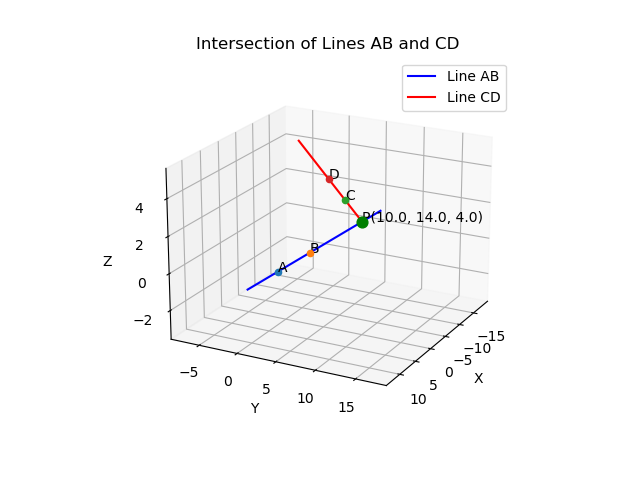
\includegraphics[width=0.75\columnwidth]{figs/8.png}
\caption{Given 2 lines are Intersecting}
\label{fig:line_eqn}
\end{figure}

\end{document}